The implemented method consists of four steps. First the given training data, which consists of video frames with labeled parts, is used to build a set of feature vectors using two descriptors. This matrix is the basis for the training of a random forest and a linear classifier. The models then classify a sliding window for the testing frames resulting in a heat map of drivable roadway. In a fourth step the generated heat map gets refined using a series of morphological operations.

\subsection{Training data} % (fold)
\label{sub:training_data}
The training data consists of two parts. First a series of eleven videos that show posed car rides with obstacles and interfering actors. The frames are present as compressed grayscale images with a size of $960\cdot 540$px. Second for each, except the first, video, a hand labeled set of positive and negative rectangle image parts. These boxes are overlapping and of varying size. As we want feature vectors of the same size the boxes are resized to a standard width of 51px. Then  the part of the corresponding frame the box bounds is gathered and the features are computed. Combined with the label this makes one testing instance.
% subsection training_data (end)

\subsection{Used features} % (fold)
\label{sub:used_features}
Two features are computed in the process of training and predicting. To describe the structural information found in the testing data a histogram of oriented gradients\cite{uoctti} (HOG) is used.
\begin{figure}[h]
	\centering
	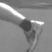
\includegraphics[height=2.5cm, width=2.5cm]{feature-image}
	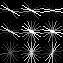
\includegraphics[height=2.5cm, width=2.5cm]{feature-hog}
	\caption{51px wide extract and its HOG}
	\label{fig:imhog}
\end{figure}
With this calculation the image is divided into overlapping blocks and on these blocks a 1-D kernel is applied vertically and horizontally. Then the pixels in the blocks are weighted and so vote for the intensity of one of nine directions of the gradients.

Furthermore we want to use the similarity of intensity distribution in positive samples and therefore add a color histogram to the feature vector. For that, pixels of the same intensity are counted and the counts are ordered by the intensity.
{\begin{figure}[h]
	\centering
	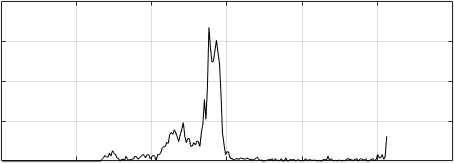
\includegraphics[width=0.95\columnwidth]{feature-hist}
	\caption{The histogram for the image in \autoref{fig:imhog}}
	\label{fig:limhist}
\end{figure}}\\
So for a box we have 9 HOG cells and with the standard of 9 orientations we get $9*31 = 279$ dimensions for the first feature. As the histogram consists of 256 values that makes in total a 535 dimensional feature vector.
% subsection used_features (end)

\subsection{Classifiers} % (fold)
\label{sub:classifiers}
I tested multiple classifiers for this task and this report describes the results with the linear classifier \texttt{LibLinear}\cite{liblinear} and with a random forest\cite{randforest}.
In a earlier stage I tried to use a not linear support vector machine (SVM) with a RBF kernel. Due to the technical limitations especially in memory it was not possible to train a model with enough data to make it usable. With change to a linear classifier I also got huge speed improvements. A linear classifier tries to find a hyperplane in the 535 dimensional feature space, the training points life in, that separates two classes. \texttt{LibLinear} is used with a L2-regularized SVM classifier as the solver. In that method the solver tries to maximize the distance between the training points and the hyperplane. A simple example of a separated set is in \autoref{fig:classifiers}(a). The significant cost of constraint violations was set at 100 through training and evaluating at a range of values. This parameter tells the classifier how many misclassifications it can accept while training so a higher cost becomes a hyperplane with smaller margins.

For the random forest the implementation from \texttt{MATLAB} is used. A random forest is a special decision tree. Decision trees classify an instance by looking at every deeper node at a feature value so that lastly all leafs are either associated with the one class or the other. A small tree is shown in \autoref{fig:classifiers}(b). This is done for all trees in the forests and the most chosen label wins. In training the tree is build by choosing a random part of the feature vector ($\sqrt{length(instance)}$) and making a split based on the best splitter. By splitting, trees are built and in the end the trees are combined to the forest which is the classifier. The number of trees is set at 30 after testing at different values.
\begin{figure}
	\centering
	\footnotesize
	\begin{tabular}{c c}
		\raisebox{-.18\height}{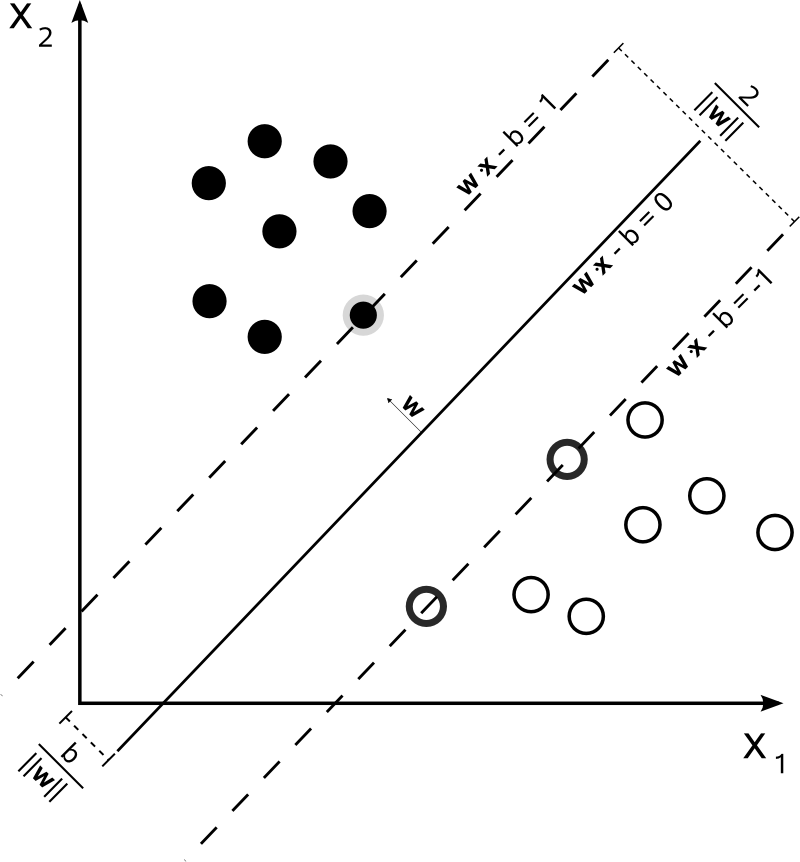
\includegraphics[width=0.4\columnwidth]{svm_example}} &
		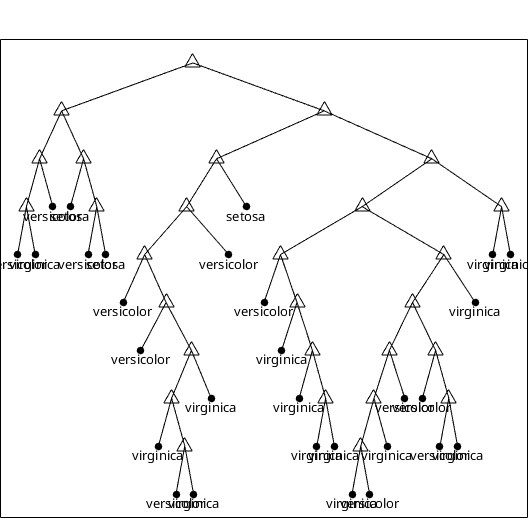
\includegraphics[width=0.4\columnwidth]{dec_tree_example} \\
		(a) line from SVM & (b) decision tree
	\end{tabular}
	\caption{Example for the classification methods}
	\label{fig:classifiers}
\end{figure}
% subsection classifiers (end)

\subsection{Computing segmentation} % (fold)
\label{sub:computing_segmentation}
The general idea to get predictions for a frame is to slide a window of varying size over the image and sum up the predicted classes. After testing I have decided for window sizes of 50, 60 and 70px. So for each of this sizes we slide the window from the top-left to the bottom-right while pushing the window by the half width after each step which makes the same sized windows overlapping. In each step the bounded image part is resized to the 51px and the HOG and histogram is calculated. After a size pass the resulting feature vectors are collected in a matrix and then passed to the predict function of the given model. For the 3 chosen sizes we then get $325 + 480 + 703 = 1508$ instances for a frame from the testing videos. To generate the heat map we now just increment the values in the belonging window of original size if the label was positive. In a last step the heat map is normalized.
% subsection computing_segmentation (end)

\subsection{Morphology} % (fold)
\label{sub:morphology}
The heat map from the predict function is not the practical result we aimed at. As one can see for example in the predicted heat map in \autoref{fig:morph_randforest}(b)
\begin{figure*}
	\centering
	\footnotesize
	\begin{tabular}{c c c}
		\gridim{I00875} & \gridim{LL_I00875_unmorph} & \gridim{LL_I00875_bw} \\
		(a) original frame & (b) prediction from classifier & (c) heat map thresholded \\[6pt]
		\gridim{LL_I00875_edge} & \gridim{LL_I00875_edge_closed} & \gridim{LL_I00875_bw_mult} \\
		(d) detected edges & (e) edges closed & (f) edges applied on heat map \\[6pt]
		\gridim{LL_I00875_bw_filt} & \gridim{LL_I00875_bw_dilated} & \gridim{LL_I00875_morph}\\
		(g) largest connected component & (h) heat map dilated & (i) result
	\end{tabular}
	\caption{\texttt{seq0002/I00875.jpg}: Prediction and morphing with \texttt{LibLinear}}
	\label{fig:morph_linear}
\end{figure*}
we get separated misclassified regions in the sky or in the houses. Also as we add up the predicted labels for the sliding windows the heat map of course is not binary but has a intensity range. Furthermore the idea with this method is to narrow the wide-scrawled predictions by using information from a edge detector. Shown in the two examples \autoref{fig:morph_linear} and \autoref{fig:morph_randforest}
\begin{figure*}
	\centering
	\footnotesize
	\begin{tabular}{c c c}
		\gridim{I00415} & \gridim{TB_I00415_unmorph} & \gridim{TB_I00415_bw} \\
		(a) original frame & (b) prediction from classifier & (c) heat map thresholded \\[6pt]
		\gridim{TB_I00415_edge} & \gridim{TB_I00415_edge_closed} & \gridim{TB_I00415_bw_mult} \\
		(d) detected edges & (e) edges closed & (f) edges applied on heat map \\[6pt]
		\gridim{TB_I00415_bw_filt} & \gridim{TB_I00415_bw_dilated} & \gridim{TB_I00415_morph}\\
		(g) largest connected component & (h) heat map dilated & (i) result
	\end{tabular}
	\caption{\texttt{seq0007/I00415.jpg}: Prediction and morphing with the random forest}
	\label{fig:morph_randforest}
\end{figure*}
you see the seven steps used on the prediction. First the normalized heat map is thresholded at a fixed value to get a binary decomposition(c). Then we compute the edges for the original frame with the canny edge detector(d). Here we ensure fine-grained edges as we assume the roadway is of few strong gradients. When we then morphologically close the edges(e), the fine-grained structures present in the surroundings of the street become ideally one face or at least of big connected components. As the heat map and the edges are present as binary images we can multiply the heat map with the complement of the edges to subtract the edges from the heat map(f). In the fifth step the largest connected component is selected and so possible lone misclassifications are discarded(g). Probably the now remaining component has fine incisions. For the last morphological step the heat map gets dilated so these small cuts at least get filled(h). The finished morphed classification is reapplied on the original frame to get a frame for the result video(i).
% subsection morphology (end)
